\chapter{Implementation} \label{chap:implementation}

\section*{}

This chapter describes the details of implementation, in particular the architecture of the tool and the database and module structure.

\section{Architecture of the solution} \label{sec:evaluation}

The solution is a module implemented on top of SCRAIM using the same technologies and infrastructures. SCRAIM is developed in the Ruby on Rails \citep{hansson2009ruby} programming language and a MySQL \citep{MySql} database. The solution uses also a new framework for charts c3js \citep{c3js}.

The architecture was designed with flexibility and extensibility in mind, so that additional practices and reference models can be easily supported in the future.

The architecture of the solution is presented in two parts: the database structure and the overall application structure (module structure).


\section{Database structure}\label{database}

The prototype was implemented inside of Scraim in order to store all the information that is generated an extension of its database was done.

For that purpose several tables in the database were created. Each one one to be flexible enough to store the information of the automatic assessments.

The tables created can be viewed in Figure \ref{fig:database}, their purpose is as follows:
\begin{itemize}
	\item \textbf{Model}
	
	This table contains the reference models agains which assessments can be made, identified by their name; in this case the only model stored is CMMI Level 2.
	\item \textbf{Area}
	
	In this table are stored the Areas; each Model must have one or more Areas.
	\item \textbf{Goal}
	
	Goals are part of the Area and each Area has one or more Goals.
	\item \textbf{Practice}
	
	Each practice is characterized by its name, a summary that gives a simplified description of the practice, its description which is more complete and with some examples in some cases and its weight. Each practice has different weights in the result of the assessment.
	
	\item \textbf{Practice Evaluation}
	
	Represent each Practice evaluation; each practice is evaluated with different criteria and is saved in the database for the presentation of the results.
	
	\item \textbf{Global Assessment}
	
	The Result of the assessment is represented by this table where it is saved the global result, which is the aggregation of all practice evaluations for the assessment.
	
\end{itemize}

\begin{figure}[!htb]
	\begin{center}
		\leavevmode
		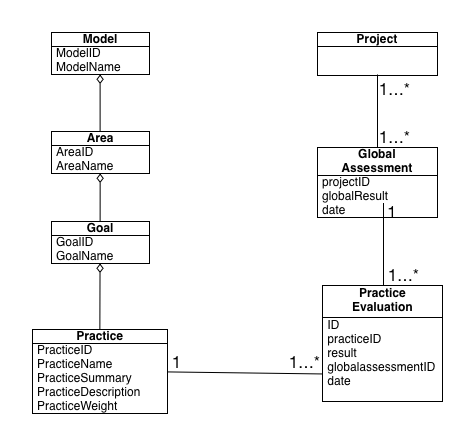
\includegraphics[width=1\textwidth]{ClassDiagram}
		\caption{Data Model of the tables added to the SCRAIM databaseTables added to database (UML class diagram)}
		\label{fig:database}
	\end{center}
\end{figure}


On the left side of the Figure \ref{fig:database}, the tables represented are those who are going to be populated with the information from the CMMI for Development and on the right side it is where the generated information is going to be stored.


\section{Module structure}

In Figure \ref{fig:esquema} we can see the overall structure of the module created.

%%explicar a estrutura
%
%
%
%\textbf{Project Info}
%This Function is called to get the project info needed to do the assessment of the practice. The information returned will ba passed through the Area Evaluator to the Practice Evaluator represented by the Abstract Evaluator.
%

\begin{figure}[H]
	\begin{center}
		\leavevmode
		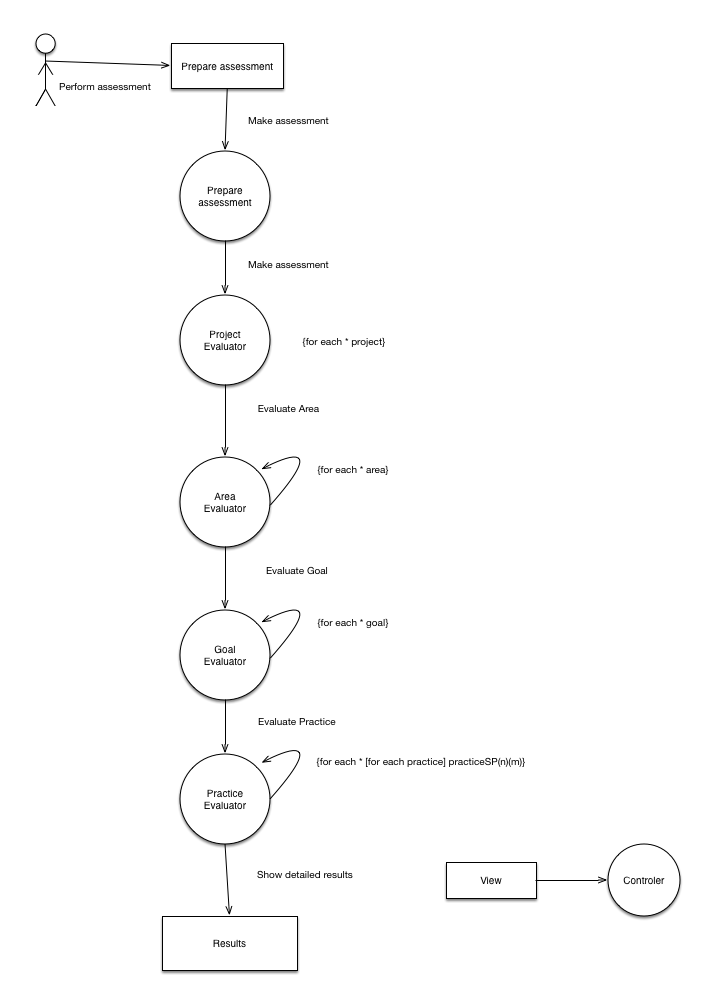
\includegraphics[width=0.9\textwidth]{umlprocess}
		\caption{Eletronic assessment process}
		\label{fig:esquema}
	\end{center}
\end{figure}

%conception

\newpage

\textbf{Prepare assessment}

Represents the view that is showed to the user to input the assessment options. It also represents the function called that validates the options selected.

\vspace{1cm}

\textbf{Make assessment}

It's the constructor and main function of the module. It calls the functions that perform the evaluation of the projects and saves the evaluations results.

\vspace{1cm}

\textbf{Project Evaluator}

For each project it is called this controller that calls each area evaluator.

\vspace{1cm}

\textbf{Area Evaluator}

This part of the module is a controller that depending of the process area, calls all the goals evaluators and receives their results.

\vspace{1cm}

\textbf{Goal Evaluator}

This evaluator is called by area evaluator; each area has one or more goals, so this is called several times for each area evaluation.

\vspace{1cm}

\textbf{Practice Evaluator}

For each practice the evaluation is different, so the function that is going to generate the result of that evaluation is different, has a different logic, but has an analogous structure. All the Practices Evaluation follow the same structure.

\vspace{1cm}

Despite the conception and the mapping of all areas from maturity level 2 of CMMI for development, this prototype only contemplates the implementation of two areas.

The Implemented areas are: Project Planning and Project Monitoring and Control.

\section{Scalability and Flexibility}

The model represented is fully capable of handling expansions of the database and the practices evaluators, the only thing needed is to follow some steps:
\begin{itemize}
	\item \textbf{Database Insertion: } It is needed to include in the file that starts the database the information of the new models (areas, goals and practices), that are going to be inserted into the tables.
	\item \textbf{Implement all Practices evaluators: } Must be implemented the rules evaluators; those evaluators are represented by the abstract evaluator.
	\item \textbf{Add to the Main Function: } The function that is going to evaluate the practices must be added to the Main Function to be called in the assessment.
\end{itemize}

After these steps the new models added are evaluated and presented in the assessment.
